
%(BEGIN_QUESTION)
% Copyright 2006, Tony R. Kuphaldt, released under the Creative Commons Attribution License (v 1.0)
% This means you may do almost anything with this work of mine, so long as you give me proper credit

Shown here is a distillation tower, used to separate a liquid mixture of substances into its constituent components.  The process of {\it distillation}, or {\it fractionation} as it is sometimes called, is very common in heavy process industries, most notably petrochemical processing:
 
$$\includegraphics[width=15.5cm]{i04681x01.eps}$$

Distillation of this nature works on the principle of different boiling points.  The distillation of alcohol (to separate a water/alcohol mix in order to obtain a purer alcohol product) is a well-known application of this technology.  In a fractionation tower, the process of boiling and condensation of the mixture's constituent components is repeated endlessly, assuring a high degree of separation between them.

The light vapors extracted from the top of a distillation tower are re-condensed into an ``accumulator'' vessel and re-introduced into the fractionation process as ``reflux.''  The heavy vapors condensing at the bottom of the tower are re-boiled into vapor form again and re-introduced into the fractionation process as ``boil-up.''  It is necessary for reflux and boil-up to be re-introduced into the tower in order to purify the final products as much as possible.  The P\&ID shown here is devoid of any instrumentation for the sake of simplicity.

\filbreak

Here, a simple reflux control loop is shown, to control the amount of reflux introduced into the tower from the accumulator:

$$\includegraphics[width=15.5cm]{i04681x02.eps}$$

Suppose the level transmitter in this system fails such that it always outputs a high (21 mA) signal.  Determine the effect this fault will have on the accumulator's liquid level.

\vskip 20pt \vbox{\hrule \hbox{\strut \vrule{} {\bf Suggestions for Socratic discussion} \vrule} \hrule}

\begin{itemize}
\item{} Judging by the symbols used in this P\&ID, what type of control system is this on the accumulator level loop (i.e. what type of signaling is used, where are the instruments located, etc.)?
\item{} Identify appropriate level measurement technologies that might be used in this application, since the diagram shown is too vague to reveal specifics.
\end{itemize}

\underbar{file i04681}
%(END_QUESTION)





%(BEGIN_ANSWER)

 
%(END_ANSWER)





%(BEGIN_NOTES)

If the transmitter fails high, the control system will ``think'' the accumulator is always full and will therefore send as much reflux flow to the tower as possible.  This will have the effect of emptying the overhead accumulator so it's real liquid level will be at or near zero at all times.

%INDEX% Measurement, level: distillation tower reflux accumulator
%INDEX% Process: distillation (generic)

%(END_NOTES)


